\documentclass[a4paper,12pt]{report}

\usepackage{alltt, fancyvrb, url}
\usepackage{graphicx}
\usepackage[utf8]{inputenc}
\usepackage{float}
\usepackage{hyperref}
\usepackage{adjustbox}
\usepackage{siunitx}
\sisetup{group-separator={\text{\space}}}

% Questo commentalo se vuoi scrivere in inglese.
\usepackage[italian]{babel}

\usepackage[italian]{cleveref}

\title{Relazione per\\``Basi di dati''}

\author{Nicolò Guerra \and
Filippo Casadei}

\begin{document}

\maketitle

\tableofcontents

\chapter{Analisi dei requisiti}

Si vuole realizzare un database per la gestione di sistemi ospedalieri. Il sistema dovrà immagazzinare dati relativi a diverse ASL,
agli ospedali ad esse associate, pazienti, medici. Dovrà registrare inoltre referti relativi a visite, interventi e appuntamenti.

\section{Intervista}
Una prima descrizione delle richieste è la seguente:
\paragraph{}
Si vuole tenere traccia dei referti prodotti nei vari ospedali delle varie ASL della regione. Un referto può essere prodotto da un
intervento o da una visita/esame. Un referto è prodotto da un medico in un ospedale, ed è riferito ad un paziente. Dei pazienti si
vuole memorizzare nome, cognome, codice fiscale, data di nascita, numero di telefono, ASL di appartenenza e referti associati.
Di un impiegato si vuole memorizzare nome, cognome, codice fiscale e ruolo. Di un medico si vuole inoltre tenere traccia dello
storico degli interventi.
Un referto viene prodotto in una specifica data e nel caso sia di un intervento, si vuole sapere la procedura, l'esito, la durata e i medici
coinvolti. Nel caso sia di una visita invece si vuole avere una breve descrizione di quest'ultima e l'eventuale terapia prescritta.
Si vogliono memorizzare inoltre i seguenti dati per gli ospedali: nome, indirizzo, ASL di appartenenza, posti disponibili e persone
che lavorano in una struttura, e se questo dispone di un pronto soccorso.
Un ospedale si compone inoltre di più unità operative, ognuna caratterizzata da un nome, un dirigente, e dal personale che vi lavora.
Ogni ospedale ha delle attrezzature, identificate da un codice di inventario e di cui si vuole memorizzare il nome e la data dell'ultima
manutenzione.
Si vogliono infine memorizzare degli appuntamenti, che possono essere ad esempio prenotazioni per interventi e coinvolgono uno o più
pazienti e uno o più medici in una certa sala dell'ospedale ad una precisa data e ora. Un medico o un paziente non possono avere più
appuntamenti nello stesso momento. Una sala non può essere occupata da 2 appuntamenti contemporaneamente.
\section{Concetti principali da modellare}
\begin{itemize}
  \item ASL: Azienda sanitaria locale, gestisce la sanità di una singola zona di competenza, solitamente provinciale
  \item Ospedale: Struttura in cui avvengono visite e interventi dei pazienti
  \item Referto: Documento prodotto da un medico come resoconto di una visita o un intervento
  \item Paziente: Persona sottoposta a trattamenti ospedalieri
  \item Medico: Persona che lavora in un ospedale (o più di uno) e effettua trattamenti
  \item Impiegato: Persona che lavora in un ospedale ma non effettua trattamenti e non può firmare referti
  \item Unità operativa (U.O.): Reparto dell'ospedale specializzato in determinati tipi di trattamenti
  \item Attrezzatura: Macchinario utilizzato per particolari interventi e/o visite
  \item Appuntamento: Programmazione di visita o intervento
  \item Visita: Consulenza con un medico riguardante lo stato di salute del paziente
  \item Intervento: Operazione ad un paziente da parte di uno o più medici
  \item Sala: Stanza in cui avvengono visite e interventi
\end{itemize}
\section{Riscrittura dell'intervista corretta}
Di un referto si vuole memorizzare la data di emissione, il paziente, i medici coinvolti e il tipo di referto, oltre ad una breve descrizione.
Se è stato prodotto per un intervento si memorizzano anche procedura, esito e durata, se invece è per una visita la terapia prescritta.

Di una persona si vogliono memorizzare nome, cognome, codice fiscale, numero di telefono.
Di un paziente inoltre si vogliono memorizzare data di nascita, ASL di appartenenza e i referti associati.
Di un impiegato si vuole memorizzare il ruolo all'interno della struttura.
Di un medico si vuole memorizzare lo storico degli interventi.

Di un ospedale si vogliono memorizzare nome, indirizzo, ASL di appartenenza, posti disponibili (inteso come capienza totale in numero di pazienti),
persone che vi lavorano e il loro numero. Si vuole inoltre sapere se l'ospedale è munito di pronto soccorso.

Di una unità operativa si vogliono memorizzare il nome, l'ospedale a cui appartiene, il dirigente, il personale che vi lavora, la capienza e i posti liberi.

Di ogni attrezzatura si vogliono memorizzare il codice di inventario, l'ospedale di cui fanno parte, il nome e la data dell'ultima manutenzione.

Di ogni appuntamento si vuole memorizzare la data e l'ora, la durata stimata, il tipo, la sala, i pazienti e i medici coinvolti. 
Un paziente e/o un medico non possono avere più appuntamenti nello stesso lasso di tempo, inoltre una sala non può essere occupata da più 
appuntamenti allo stesso tempo.
\section{Principali azioni richieste}
\begin{itemize}
  \item Aggiungere un nuovo ospedale
  \item Aggiungere una nuova unità operativa
  \item Rimuovere un'unità operativa da un ospedale
  \item Aggiungere un nuovo paziente
  \item Aggiungere un nuovo impiegato/medico
  \item Fissare un appuntamento
  \item Cancellare un appuntamento
  \item Cambiare la data e/o il luogo di un appuntamento
  \item Aggiungere un nuovo referto
  \item Ricercare i referti per medico o per paziente
  \item Aggiungere nuova attrezzatura
  \item Rimuovere attrezzatura
  \item Aggiornare la data di manutenzione di un'attrezzatura
  \item Ricerca di unità operative all'interno di un ospedale
  \item Ricerca di ospedali appartenenti ad un'ASL specifica
  \item Aggiungere una sala ad un ospedale
  \item Rimuovere una sala da un ospedale
  \item Ricercare ospedali con posti liberi in una determinata unità operativa
\end{itemize}

\chapter{Progettazione concettuale}
\begin{figure}[H]
	\centering{}
	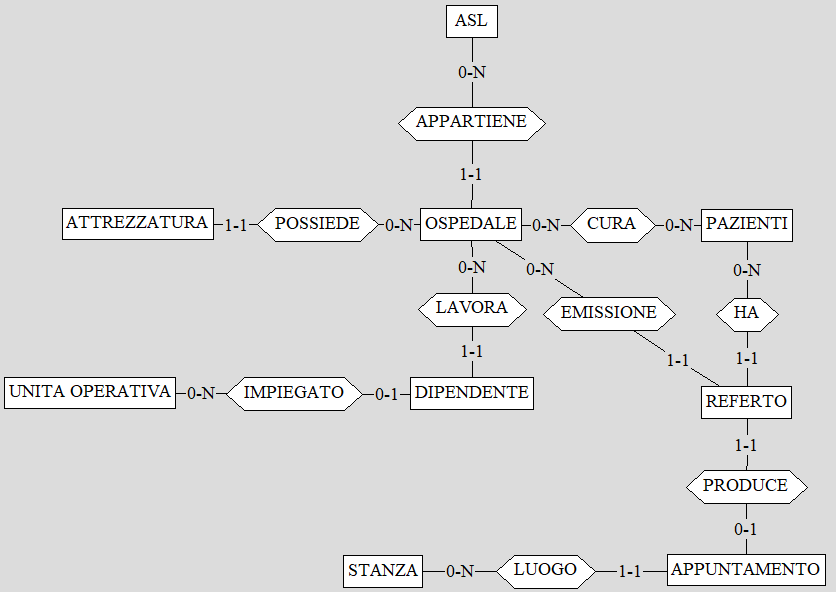
\includegraphics[width=\textwidth]{img/scheletro.png}
	\caption{Schema scheletro del problema.}
	\label{img:scheletro}
\end{figure}
Dopo l'esame del dominio del problema risultano alcune considerazioni da fare, che implicano diversi raffinamenti possibili:

Va considerata la presenza di diverse categorie di lavoratori all'interno di un ospedale e solo alcuni di questi devono essere in grado di rilasciare
referti ai pazienti. Per questi motivi si è deciso di dividere l'entità dipendenti dello schema scheletro in amministrativi e personale sanitario, che assieme a pazienti
risultano essere sottocategorie dell'entità persona, identificabili mediante codice fiscale.

Inoltre unicamente gli amministrativi sono collegati direttamente all'ospedale, mentre il personale sanitario si relaziona ad un'unità operativa, quest'ultima associata 
ad un ospedale.

Gli appuntamenti vengono modellati come entità perché devono essere identificati da data, ora e luogo in cui avvengono, attributi propri dell'appuntamento 
stesso. Non risultano però modellabili alcuni requisiti. Essendo gli appuntamenti protratti nel tempo non si può modellare nello schema E-R il vincolo di 
non poter avere 2 appuntamenti sovrapposti. Diversamente da come descritto sopra un appuntamento non è direttamente connesso ad un referto, ma esprime
unicamente il concetto di incontro tra un pazienti e medici.

Anche visite e interventi sono estensioni della generica entità referto, ne rappresentano infatti il tipo, e i dati specifici per l'uno o per l'altro caso. Inoltre per
poter ricostruire lo storico degli interventi di un medico ogni referto è anche associato al medico che lo ha prodotto.

È stata anche aggiunta la relazione di registrazione di un paziente presso una determinata ASL.

Lo schema E/R definitivo risulta quindi essere il seguente:
\begin{figure}[p]
  \begin{adjustbox}{addcode={\begin{minipage}{\width}}{\caption{%
    Schema E/R del problema.
    }\end{minipage}},rotate=270,center}
    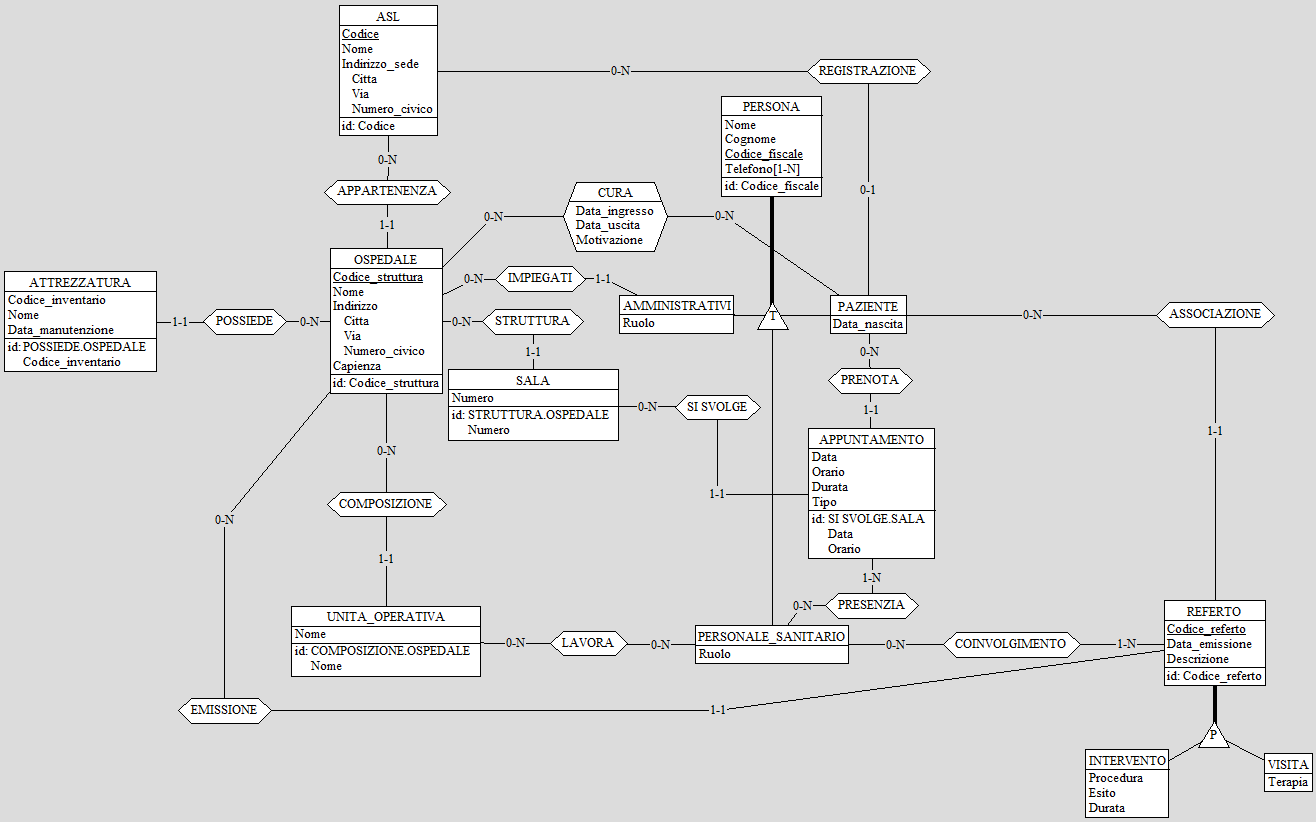
\includegraphics[height=0.93\textwidth]{img/er_final.png}
    \label{img:er}
  \end{adjustbox}
\end{figure}

\chapter{Progettazione logica}
\section{Stima del volume dei dati}
Si stimano nella tabella seguente il volume dei dati previsto nel database:
\subsection{Entità}
\begin{center}
  \begin{tabular}{ c | S[table-format=8.0, table-space-text-pre=(, table-space-text-post=)] }
    Nome & Quantità \\
    \hline
    Amministrativi & 40000 \\
    Appuntamento & 1000000 \\
    ASL & 100 \\
    Attrezzatura & 15000 \\
    Intervento & 200000 \\
    Ospedale & 1000 \\
    Paziente & 50000000 \\
    Persona & 51000000 \\
    Personale sanitario & 500000 \\
    Sala & 30000 \\
    Unità operativa & 10000\\
    Visita & 700000 \\
  \end{tabular}
\end{center}
 
Va considerato che essendo Personale sanitario, Amministrativi e Paziente gerarchie di persona il loro volume è 
sovrapposto (la copertura è totale ma non esclusiva). 
Anche Intervento e Visita sono gerarchie di Referto, ma essendo questa volta una copertura totale e disgiunta Referto
è stato omesso perché ricavabile come somma di queste 2.
I volumi di Intervento e Visita sono inoltre calcolati su un anno di operatività. Questo perché sono dati che crescono molto rapidamente 
e si rende necessario un sistema di archiviazione a lungo termine per evitare di sovraccaricare il sistema e causare inefficienze.

\subsection{Relazioni}
\begin{center}
  \begin{tabular}{ c | S[table-format=8.0, table-space-text-pre=(, table-space-text-post=)] }
    Nome & Quantità \\
    \hline
    Appartenenza & 1000 \\
    Associazione & 900000 \\
    Coinvolgimento & 1300000 \\
    Composizione & 10000 \\
    Cura & 6000000 \\
    Emissione & 900000 \\
    Impiegati & 40000 \\
    Lavora & 700000 \\
    Possiede & 15000 \\
    Prenota & 1000000 \\
    Presenzia & 1500000 \\
    Registrazione & 45000000 \\
    Si svolge & 1000000 \\
    Struttura & 30000 \\
  \end{tabular}
\end{center}

Si consideri che come nella sezione precedente anche qui alcuni dati sono stati stimati su un anno di operatività. 
Cura è una relazione che cambia rapidamente nel tempo e per evitare il sovraccarico del sistema va archiviata a intervalli regolari.

\end{document}